\section{Victor Hamburger}\label{victor-hamburger}

Tags: NPC Creatore: Lorenzo Luogo: Goldendoor

\section{{[}Nome{]}}\label{nome}

\begin{center}\rule{0.5\linewidth}{0.5pt}\end{center}

\begin{figure}
\centering
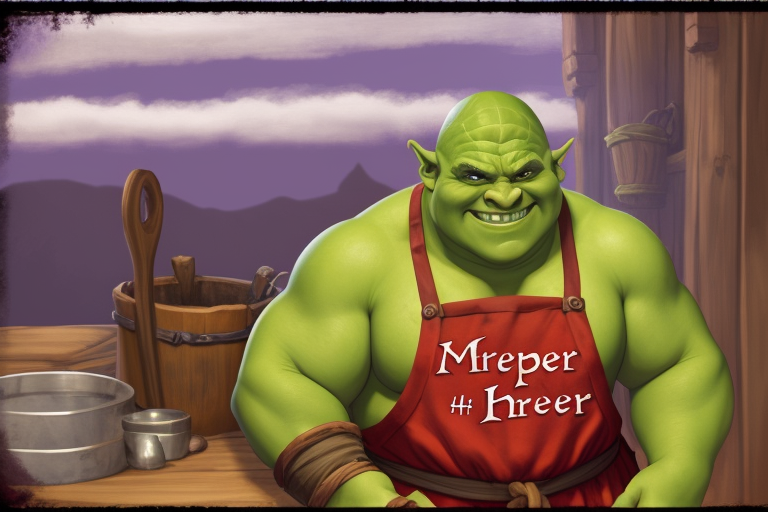
\includegraphics{orc-innkeeper-he-is-smiling-he-has-a-red-apron-with-drunk-ogre-written-on-it-he-is-a-orc-like-s.png}
\caption{orc-innkeeper-he-is-smiling-he-has-a-red-apron-with-drunk-ogre-written-on-it-he-is-a-orc-like-s.png}
\end{figure}

Informazioni Generali

Età: 40

Data di nascita: 1984

Luogo di nascita: Forregard

Razza: Orco

Classe: Guerriero

Alleati: Leona, Hakram

Nemesi:

Alias:

Professione: Locandiere

\begin{center}\rule{0.5\linewidth}{0.5pt}\end{center}

\subsection{1. Descrizione Generale}\label{descrizione-generale}

\begin{center}\rule{0.5\linewidth}{0.5pt}\end{center}

\begin{figure}
\centering
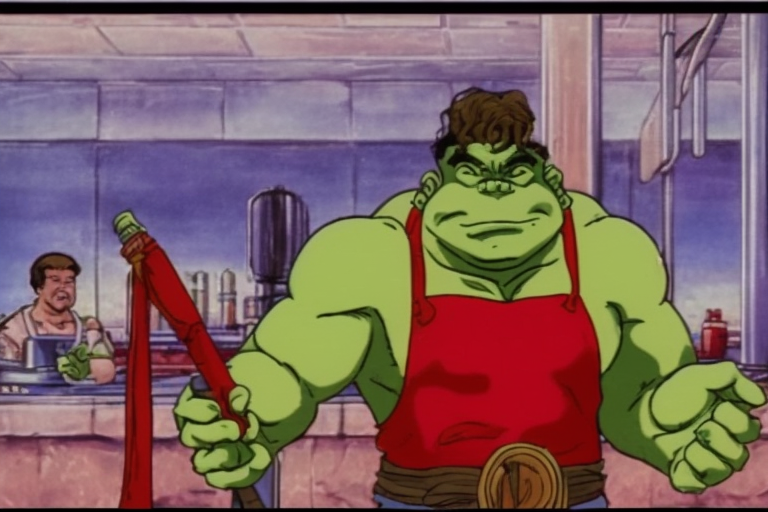
\includegraphics{retroanime-style-orc-innkeeper-he-is-smiling-he-has-a-red-apron-with-drunk-ogre-written-on-it-.png}
\caption{retroanime-style-orc-innkeeper-he-is-smiling-he-has-a-red-apron-with-drunk-ogre-written-on-it-.png}
\end{figure}

Victor è il gestore della locanda dell'Orco Ubriaco. È un orco con una
stazza imponente e un volto segnato dall'età e dall'esperienza. Ha la
pelle verde e un paio di occhi profondi e penetranti. Sono anni che
dedica l'anima e il cuore a gestire l'Orco Ubriaco, rendendolo un punto
di riferimento per il quartiere.

\begin{quote}
\emph{Se paghi, mangi. Se non paghi, mangi e lavi i piatti!}
\end{quote}

\subsection{2. Biografia}\label{biografia}

\begin{center}\rule{0.5\linewidth}{0.5pt}\end{center}

La storia di Victor è legata all'Orco Ubriaco, la locanda che gestisce
da molti anni. Originario della Nortandria, regione del Nord Valtara, ha
ereditato l'attività da un lontano zio, e ha deciso di abbandonare la
carriera militare per dedicarsi alla cucina. Nonostante la sua possenza
fisica (ama allenarsi) possa intimorire a prima vista, Victor è noto per
la sua gentilezza e la sua disponibilità verso coloro che si ritrovano
nella sua locanda.

\subsection{3. Carriera}\label{carriera}

\begin{center}\rule{0.5\linewidth}{0.5pt}\end{center}

In giovinezza ha prestato servizio come militare in diverse città
Valtaresi, ma da quando è diventato il proprietario della locanda,
Victor ha dedicato anima e cuore alla gestione dell'Orco Ubriaco. La
locanda è diventata un punto di ritrovo per avventurieri, mercanti e
viaggiatori, ma anche per ladri, furfanti e guardie cittadine. Il suo
approccio caloroso e accogliente ha contribuito al successo duraturo del
locale, diventato un rifugio unico all'interno della splendende e
decadente città di Goldendoor.

\subsubsection{3.1 La Locanda dell'Orco
Ubriaco}\label{la-locanda-dellorco-ubriaco}

Le porte della locanda si aprono a chiunque ne batta il battente,
indipendentemente da provenienza o status. Dentro quelle mura, ogni
rigido confine sociale si dissolve, e la locanda diventa un teatro dove
le maschere del mondo esterno vengono gettate via.

Il sorriso di Victor accoglie chiunque: re o straccione, mercante o
ladro, tutti sono ospiti graditi, purché possano pagare (o lavare i
piatti).

All'interno di questa tana di contraddizioni, gli avventurieri narrano
storie sotto la luce fioca delle candele, i mercanti contrattano sotto
lo sguardo vigile di Victor, e i viaggiatori trovano rifugio nei loro
pensieri. Nel contempo, ladri e ricercati trovano un po di calma, e le
guardie cittadine abbandonano il peso delle leggi e dei doveri,
immergendosi nella folla come semplici avventori.

L'Orco Ubriaco è più di una locanda; è un crocevia di storie, un porto
sicuro per gli esuli della società e un rifugio per coloro che cercano
un attimo di tregua dai rigidi ruoli della vita. Nell'oscurità di questa
taverna, Victor preserva un'armonia fragile, dove le leggi non scritte
sono tanto importanti quanto il banchetto che si svolge sotto il suo
tetto.

\subsection{4. Personalità}\label{personalituxe0}

\begin{center}\rule{0.5\linewidth}{0.5pt}\end{center}

Victor è un individuo affabile e aperto. Nonostante la sua stazza, è
noto per la sua gentilezza e disponibilità. È un ascoltatore attento e
spesso si trova ad essere un confidente per i suoi clienti. Ha un
profondo senso di lealtà nei confronti della clientela, che considera
come una famiglia allargata. Negli ultimi tempi, Victor è stato
coinvolto in un segreto che coinvolge la principessa Leona e il suo
amato Hakram. Ha fornito loro rifugio all'Orco Ubriaco, coprendo le loro
azioni e proteggendo il loro segreto. La sua determinazione nel
sostenere la fuga di Leona è stata motivata dalla sua compassione e dal
desiderio di aiutare coloro che cercano di sfidare le convenzioni e
seguire il proprio cuore: se Victor non avesse seguito il suo cuore, a
quest'ora sarebbe ancora un triste militare, e sarebbe morto da triste
militare, proprio come suo padre!

\subsection{A. Coinvolgimenti in Eventi
Recenti}\label{a.-coinvolgimenti-in-eventi-recenti}

\begin{center}\rule{0.5\linewidth}{0.5pt}\end{center}

\href{Untitled\%20Database\%209d3373b6ca9142f882c6d111e68562cb.csv}{Untitled
Database}

\subsection{B. Aggiornamenti}\label{b.-aggiornamenti}

\begin{center}\rule{0.5\linewidth}{0.5pt}\end{center}

\href{Untitled\%20baa9073e37d4412cb819296252ad4947.csv}{}
